\chapter{Extendiendo RISC-V}

Este capítulo explica los pasos seguidos para diseñar un acelerador de BNN, como se ha incluido en una CPU RISC-V y los resultados que se han obtenido al utilizarlo.

\section{Diseño del acelerador}

Como se ha explicado en secciones previas, la sección del algoritmo mas importante a optimizar es el muestreo de distribuciones gaussianas. Para ello se va incluir un GRNG como una nueva unidad funcional (UF) en la CPU RISC-V base. Sarwar Malik \emph{et al.} \cite{clt_grng} propusieron un diseño basado en el TCL que añadía un componente corrector para reducir el error de muestreo de las colas de la distribución. Como también se ha mostrado previamente, no es necesaria una gran precisión a la hora de muestrear distribuciones, por lo que se va a diseñar un GNRG basado en la suma de 12 distribuciones uniformes sin bloque corrector.

\subsection{Generación de números pseudoaleatorios uniformes}

Para generar números pseudoaletorios uniformes se ha utilizado un componente hardware llamado \textit{\textbf{L}inear \textbf{F}eedback \textbf{S}hift \textbf{R}egister} (LFSR). Se basan en un circuito de retroalimentación y un registro de estado. El circuito de retroalimentación es un conjunto de puertas XOR que implementan un polinomio generador. Dado un registro de estado de $n$ bits, si el polinomio puede producir $2^n-1$ valores antes de empezar a repetir la secuencia entonces la secuencia es máxima. Alfke \cite{lfsr_poly} recopiló una lista de polinomios generadores para secuencias máximas para varios tamaños de registros de estado. La desventaja de este tipo de LFSR es que no pueden generar más de un bit con baja correlación entre muestras. La Figura \ref{fig:lfsr_bar_corr} muestra diagramas de muestras con alta correlación.

\begin{figure}[h]
    \centering
    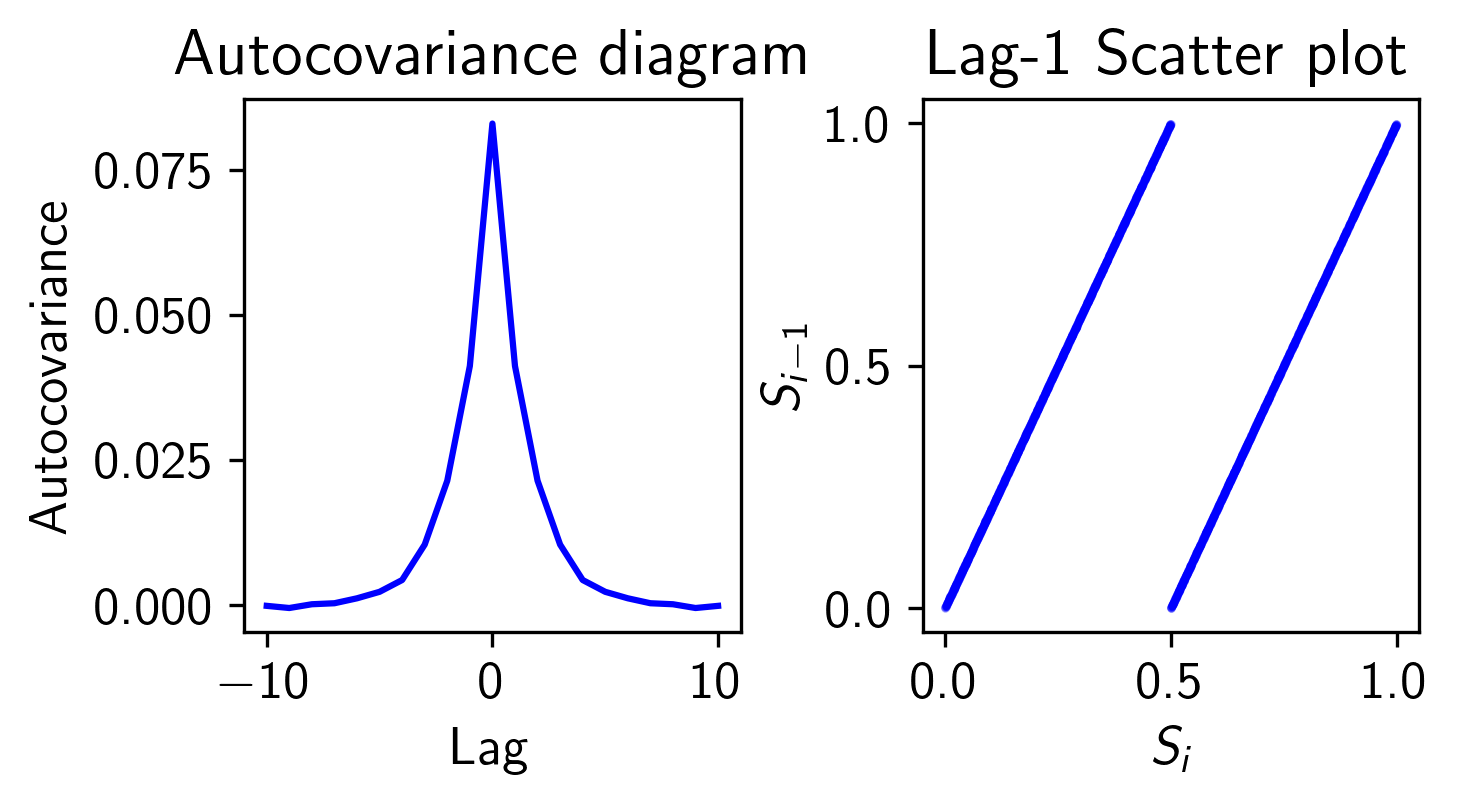
\includegraphics[width=0.7\textwidth]{root/Imagenes/5_riscv/lfsr_bar_corr.png}
    \caption{Diagramas de correlación de $10^4$ muestras de 12 bits de un LFSR. A la izquierda un diagrama de autocovarianza para diferentes distancias entre muestras. A la derecha un diagrama de dispersión de una muestra $i$ y la $i-1$.}
    \label{fig:lfsr_bar_corr}
\end{figure}

Para paliar este problema se ha utilizado un \textit{Lookahead} LFSR \cite{look_ahead_lfsr_base}. Estos LFSR tienen un circuito de retroalimentación más complejo que generan $n$ bits con baja correlación. Este circuito aplica el polinomio generador base $n$ veces, Colavito \emph{et al.} \cite{look_ahead_lfsr_design} detallan como obtener estos circuitos mediante exponenciación de matrices y que restricciones deben seguir. En este trabajo se ha desarrollado un \textit{script} en Python que genera código VHDL para implementar \textit{Lookahead} LFSR utilizando su método. La Figura \ref{fig:lfsr_good_corr} muestra los diagramas de correlación que se obtienen utilizando este tipo de LFSR.

\begin{figure}[h]
    \centering
    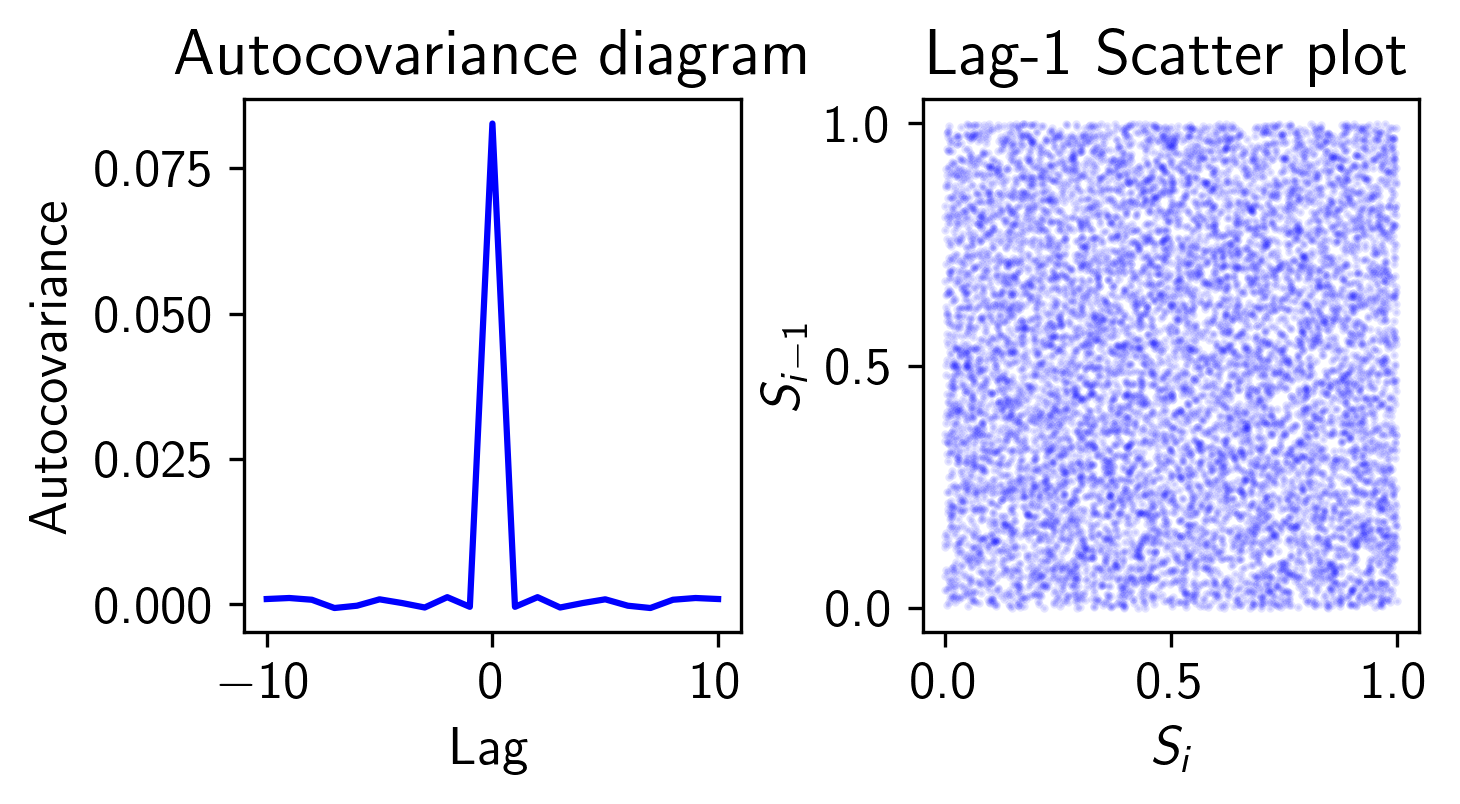
\includegraphics[width=0.7\textwidth]{root/Imagenes/5_riscv/lfsr_good_corr.png}
    \caption{Diagramas de correlación de $10^4$ muestras de 12 bits de un 12-\textit{Lookahead} LFSR. A la izquierda un diagrama de autocovarianza para diferentes distancias entre muestras. A la derecha un diagrama de dispersión de una muestra $i$ y la $i-1$.}
    \label{fig:lfsr_good_corr}
\end{figure}

\subsection{Generador de números pseudoaleatorios gaussianos}

Un GRNG basado en el TCL tiene 2 componentes principales, un generador de muestras de distribuciones uniformes y un árbol de sumadores que las acumula. Para sumar 12 muestras se necesita un árbol de 4 niveles. Como se busca obtener una muestra final de 16 bits las muestras iniciales deben ser de 12 bits, ya que por cada nivel del árbol las muestras aumentan su tamaño en 1 bit para evitar problemas de desbordamiento. Para evitar afectar negativamente a la frecuencia del reloj de la CPU original el árbol se ha segmentado por niveles, lo que permite obtener una muestra por ciclo. Solamente penalizando en el cambio de semilla, que hay que esperar 4 ciclos para obtener muestras con la semilla actualizada.

Para generar 12 muestras de 12 bits se utiliza un 144-\textit{Lookahead} LFSR con un registro de estado de 151 bits. Las muestras representan valores entre 0 y 1, codificados en coma fija con una escala $2^{12}$. Para centrar la muestra final se utiliza un restador de 16 bits con un valor constante $6 \cdot 2^{12}$. La Figura \ref{fig:grng} muestra un diagrama del diseño y la Figura \ref{fig:grng_state} la máquina de estados de su unidad de control.

\begin{figure}[h]
    \centering
    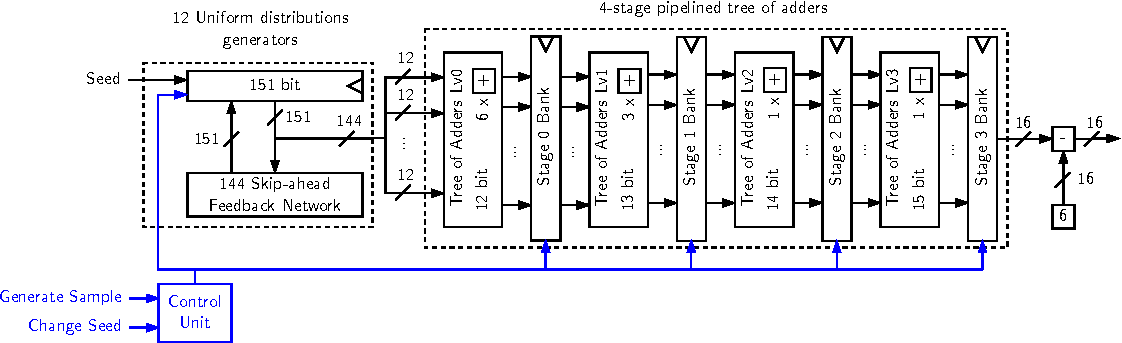
\includegraphics[width=\textwidth]{root/Imagenes/5_riscv/grng.pdf}
    \caption{Diagrama del GRNG implementado. Las señales de control se muestran en azul, el resto en negro.}
    \label{fig:grng}
\end{figure}

\begin{figure}[h]
    \centering
    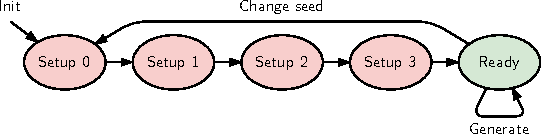
\includegraphics[width=0.8\textwidth]{root/Imagenes/5_riscv/grng_states.pdf}
    \caption{Diagrama de estados de la unidad de control del GRNG. El estado en el que se pueden generar muestras válidas esta marcado en verde, el resto en rojo.}
    \label{fig:grng_state}
\end{figure}

\section{Modificaciones al procesador}

El GRNG diseñado se ha integrado en la CPU original como una nueva UF en la etapa \textit{Execute}. Para ello se ha modificado la etapa de \textit{Decode} para añadir 2 nuevas instrucciones y el selector de resultado de la etapa \textit{Execute}. La Figura \ref{fig:extended_riscv_core} muestra un diagrama de la ruta de datos 

\begin{figure}[h]
    \centering
    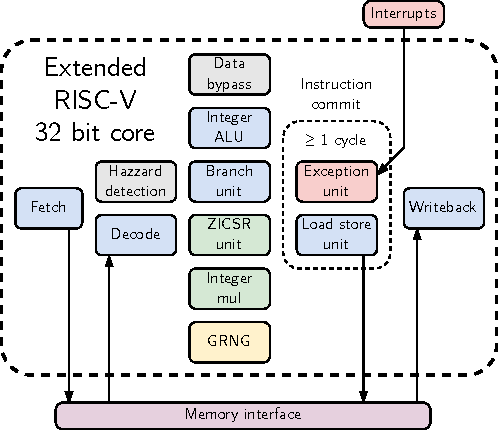
\includegraphics[width=0.75\textwidth]{root/Imagenes/5_riscv/extended_core.pdf}
    \caption{Ruta de datos del procesador RISC-V extendido con el GRNG.}
    \label{fig:extended_riscv_core}
\end{figure}

Otra opción posible habría sido añadirlo como un periférico que se accediera mediante entrada y salida mapeada en memoria (\textit{\textbf{M}emory \textbf{M}apped \textbf{I}nput \textbf{O}utput}), pero esta fue descartada por los siguientes motivos. Implicaría que se accedería mediante instrucciones \texttt{load} y \texttt{store}, lo que reduciría el rendimiento ya que estas instrucciones no permiten consumidores a distancia 1. Además el acceso a memoria generalmente requiere circuitos mas complejos por lo que estas instrucciones pueden tener un coste mas elevado, esto no ocurre en la CPU base, cuyo acceso a memoria es lo más simple posible, pero esto si que podría ocurrir en otras CPU y afectar negativamente al rendimiento. Otro factor en contra de esta aproximación es que en el futuro se quiere crear una UF mas compleja que utilice el GRNG.

\subsection{Actualizar el compilador}

Para poder utilizar el GRNG se han añadido 2 instrucciones nuevas al repertorio RISC-V. El objetivo de estas nuevas instrucciones es acelerar el motor de inferencia que se ha desarrollado, por lo que se han de poder utilizar desde código de alto nivel en C. Por lo que se ha actualizado el compilador \texttt{gcc} para RISC-V, lo que se ha podido hacer gracias a que es de código abierto. A continuación se describen las instrucciones añadidas:
\begin{itemize}
    \item \texttt{setseed rs1}. Cambia la semilla por el valor del registro \texttt{rs1}.
    \item \texttt{genum rd}. Genera una muestra de $\mathcal{N}(0,1)$ y la guarda en los 16 bits mas altos del registro \texttt{rd}. Eso implica que la muestra está codificada en coma fija en escala $2^{12 + 16}$.
\end{itemize}

Para poder actualizar el compilador hay que definir la codificación de las instrucciones siguiendo las directrices de RISC-V. Además hay que definir una máscara junto con un valor para que \texttt{gcc} pueda comprobar la codificación mediante una operación \texttt{and}. Para ambas instrucciones se ha utilizado la codificación de instrucciones tipo R de RISC-V y se muestran en las Tablas \ref{tab:code_setseed} y \ref{tab:code_genum}.

\begin{table}[h]
    \centering
    \caption{Codificación, máscara y validación de la instrucción \texttt{setseed} separada en los campos de instrucción RISC-V tipo R.}
    \label{tab:code_setseed}
    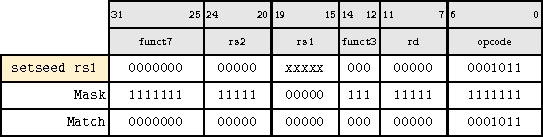
\includegraphics[width=0.85\textwidth]{root/Imagenes/5_riscv/code_setseed.pdf}
\end{table}

\begin{table}[h]
    \centering
    \caption{Codificación, máscara y validación de la instrucción \texttt{genum} separada en los campos de instrucción RISC-V tipo R.}
    \label{tab:code_genum}
    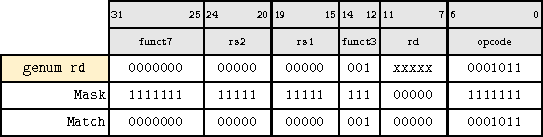
\includegraphics[width=0.85\textwidth]{root/Imagenes/5_riscv/code_genum.pdf}
\end{table}

%%%%%

\section{Análisis de resultados}

\subsection{Análisis de coste}
\todo pequeña introduccion de que es una FPGA quizas aqui

implementacion en FPGA utilizando Xilinx ZCU104 FPGA board: 240 Look-Up Tables (LUT) and 320 Flip-Flops (FF). Power measurements where obtained using the power report of Vivado Design suite. %, which implies a 9.86 and a 16.65\% increment for LUT and FF, respectively, over our small base CPU. 
This cost includes the GRNG and the modifications of the CPU instruction decoding and the data pipeline. These modifications have no impact on the 100 MHz clock, and only increase the power consumption by 0.65\%. Therefore, the reduction in energy consumption is almost identical to the performance gain. 

\begin{table}[ht]
\centering
\caption{FPGA resource utilization and power consumption of the baseline RISC-V CPU and the GRNG extension.}
\label{tab:riscv_fpga_utilization}
\begin{tabular}{lrrr}
\hline
& \multicolumn{2}{c}{\textbf{Resource Utilization}} & \textbf{Utilization \%}\\
\textbf{Type} & \textit{Base CPU} & \textit{GRNG Extension} & \textit{Extended CPU}\\ \hline
LUT	        & 2435 & 240 & 1.16 \\
Flip-Flop	& 1922 & 320 & 0.49 \\
BRAM	    & 16   & 0 & 5.13 \\
DSP	        & 12   & 0 & 0.69 \\ \hline
 & \multicolumn{3}{c}{\textbf{Power consumption (W)}} \\
\textbf{Type} & \textit{Base CPU} & \textit{GRNG Extension} \\ \hline
Dynamic & 0.023 & 0.004 \\
Static & 0.593 & 0 \\ \hline
\end{tabular}
\end{table}

